% coding:utf-8

\section{Bestückung}

\subsection{Bestückungsplan}
\begin{figure}[h!]
	\centering
	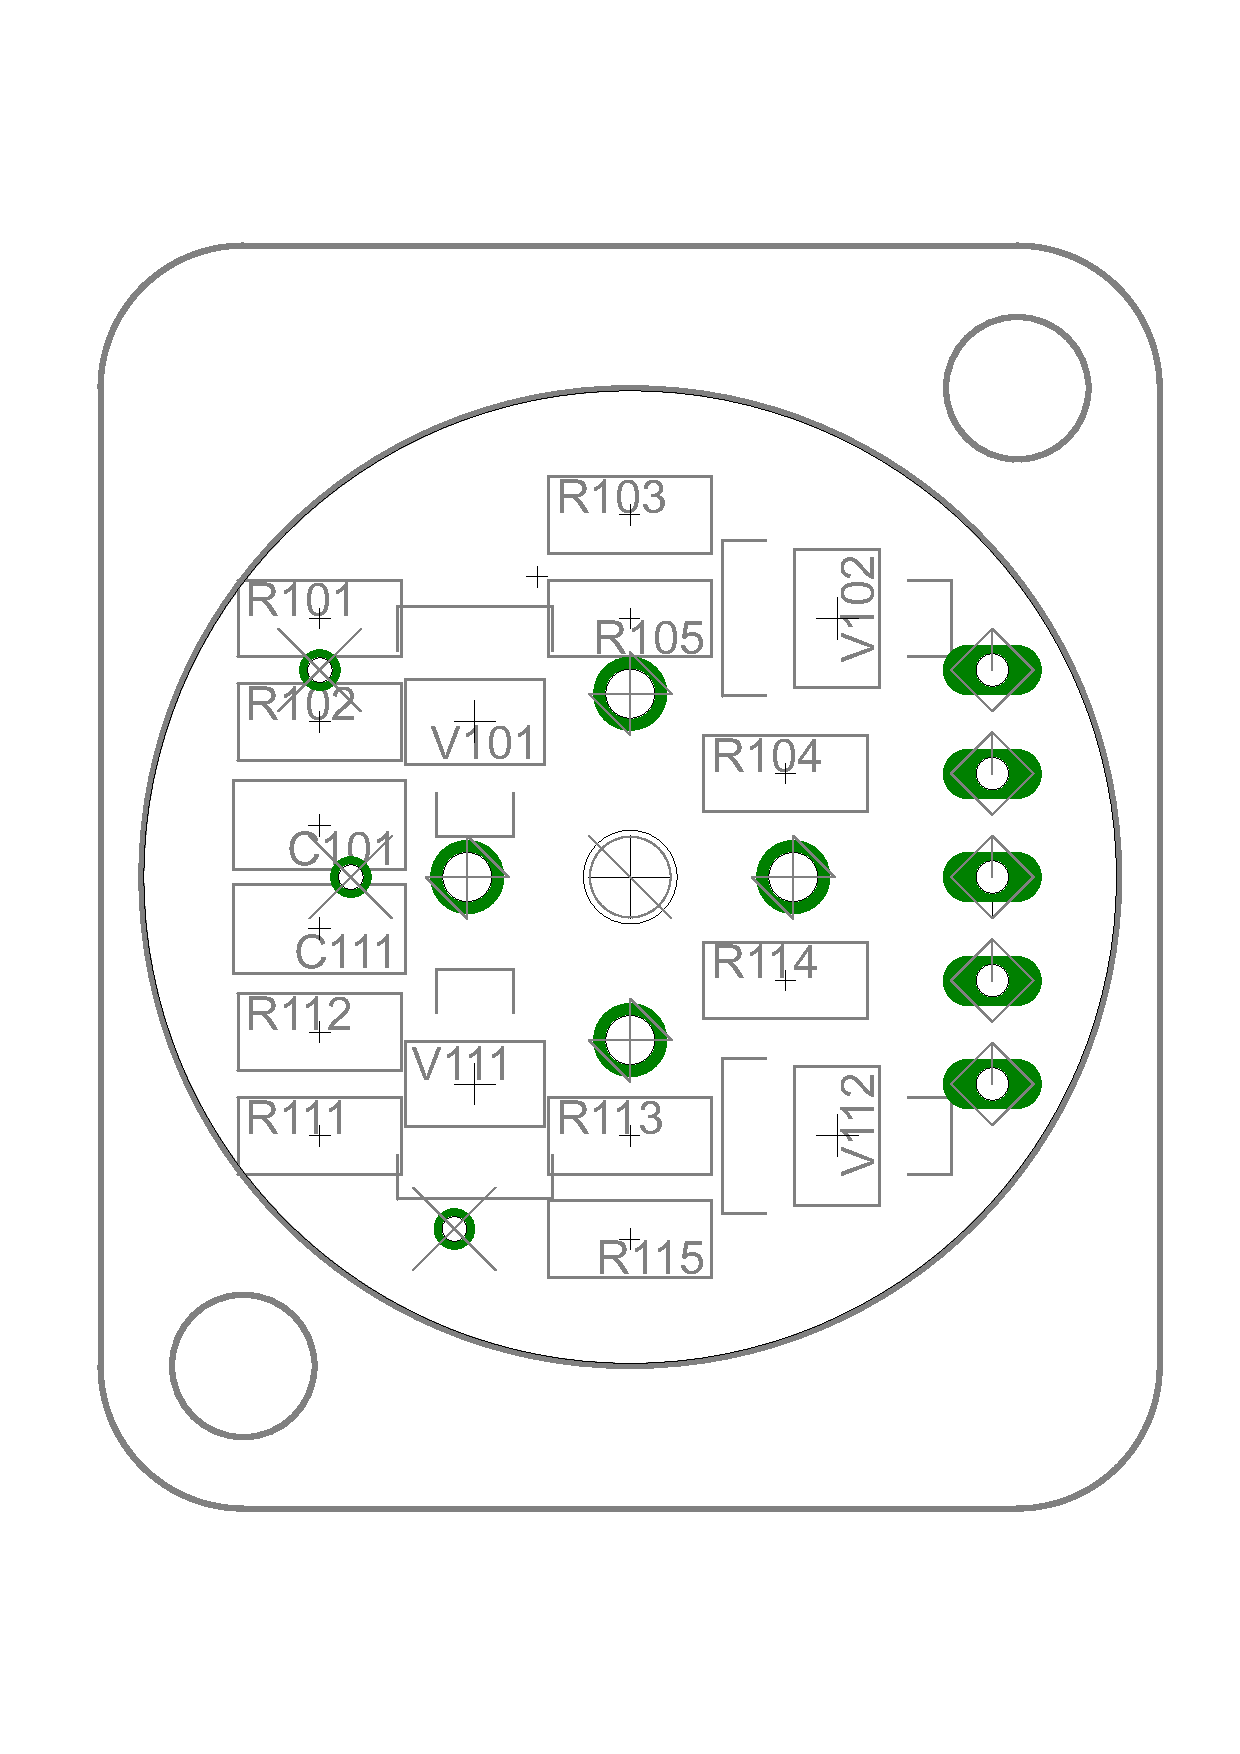
\includegraphics[scale=\layscale]{fig/xlr_pegelwandler_v_1_2_best_eagle.pdf}
	\caption{Bestückungplan V1.2}
	\label{fig:best}
\end{figure}


\subsection{Vorgehen}
Zunächst werden alle oberflächenmontierten Bauteile und die Stiftreihe für den 
Anschluss an das Arduino nach Bestückungsplan (Abbildung \ref{fig:best}) 
bestückt. Anschliessend kann die Platine an den XLR-Stecker gesteckt und an 
diesem verlötet werden. 